\documentclass[10pt,preprint,onecolumn]{article}
\usepackage[utf8]{inputenc}
\usepackage[english]{babel}
\usepackage[T1]{fontenc}
\usepackage{mathtools, comment, url, hyperref}
\usepackage[cm]{fullpage}
\usepackage{setspace}
\usepackage{float}
\usepackage{wrapfig}
\usepackage[pdftex]{graphicx}
\usepackage{tikz}
\usetikzlibrary{trees}
\usepackage{caption}
\usepackage{cite}
\usepackage{subcaption}
\usepackage{lscape}
\restylefloat{figure}
\singlespacing

\begin{document}

\part{Underground Mining}
%% proceso de extraccion, limitaciones fisicas, logicas, movilidad
%% no gps, priorizacion, alertas, nodos heterogeneos



% underground mining background
\section{Communications in Underground Mining}
Para determinar la comunicación existente y posible en minería, es necesario separar la minería de rajo abierto, que suele contar con redes celulares negociadas directamente con los proveedores de internet  ---exceptuando aquellas de pequeña escala y artesanal---, y la minería subterránea, donde no existen los medios de comunicación disponibles en la superficie. Por esto, ha surgido tecnología dedicada a la minería subterránea, que a su vez cuenta con una gran variabilidad de ambientes como túneles y galerías. A continuación se presenta una revisión de las características más importantes en estos ambientes, tomadas del estudio realizado por Mauricio Contreras \cite{tesis} de comunicación en minas chilenas subterráneas, y del informe interno de Codelco para Intraestructura en Minas Subterráneas\cite{doccodelco}.

\section{Características Importantes}

La comunicación en minería es fundamental para la coordinación de actividades, imprescindible para evitar accidentes que pueden ser fatales. Se hace énfasis a la comunicación de seguridad, tanto de datos tomados por sensores como de alertas para notificar un potencial problema humano que podría desencadenar una falla de mayor escala.

\begin{enumerate}
\item \textbf{Robustez:} Dado que las minas subterráneas están sujetas a potenciales colapsos y otros riesgos, la habilidad de un equipo de comunicación de emergencia de mantenerse operacional ante un accidente es fundamental. Por ello, se requiere una infraestructura de red que no se desconecte con un daño estructural.

\item \textbf{Flexibilidad:} El ambiente de las minas está continuamente cambiando por el proceso de extracción. Esto resulta en una necesidad continua de expandir y modificar la conectividad necesaria. Los sistemas que requieren un gran esfuerzo de instalación ofrecen una menor flexibilidad, pero a la vez, un sistema totalmente inalámbrico puede congestionarse al expandirse el sistema.

\item \textbf{Rango/Cobertura:} Dadas las distancias potencialmente largas entre los operarios, y el hecho de que la topología de la mina es complicada y cambiante, es necesaria una alta cobertura en las distintas ubicaciones donde puedan estar desarrollándose las actividades. Los sistemas de radio, ampliamente utilizados en minería, poseen un alcance bajo al estar bajo tierra.
\end{enumerate}

\section{Comunicación actual}
En la actualidad, existen topologías de red principalmente cableadas en minas subterráneas, especialmente en aquellas donde la operación es guiada remotamente, por lo que se requiere una conectividad en tiempo real para obtener un desempeño óptimo. Aún así, existen diversas zonas y niveles de varios kms de longitud donde no existe conectividad más allá de las radios portadas por equipos de operarios.

Existe un espectro de frecuencias (entre 600 y 3000Hz) que permite una propagación de señal de radio a distancias considerables a través de la tierra (\emph{Through the Earth} o TTE), pero requieren la instalación de antenas muy grandes, por lo que necesitan un espacio grande para ser instaladas. Estas suelen brindar comunicación en una dirección, usando una antena grande en el exterior y equipos pequeños sobre los operarios, que pueden recibir información en caso de emergencias tal como las áreas afectadas o las rutas de escape.

El uso de radios entre operarios es basado en Push-To-Talk (PTT), donde los operarios deben sintonizar un mismo canal, y presionar un botón para hablar, y luego soltándolo para escuchar. Las radios usualmente permiten varios canales, pudiendo sincronizar grupos a través del uso de éstos. 

Es también común dividir a los usuarios, desde una perspectiva de comunicación, por sus unidades jerárquicas (como mantenimiento, operaciones, supervisores, etc). Una unidad jerárquica puede poseer uno o más canales asignados. Cabe mencionar que las distintas unidades conviven en los mismos espacios, pero el alto ruido ambiental y las orejeras utilizadas por ello hacen que no fluya información entre los distintos grupos.

Estos factores generan segregación de operarios en grupos pequeños (al alcance de radio) y divididos por jerarquías, que sólo obtienen información desde el exterior, sin poder notificar el estado actual de la zona entre sí ni hacia el exterior.
% specific codelco needs and 
\section{Codelco's requirements}
\part*{Requerimientos}
Antes de comparar protocolos, resulta interesante analizar cuáles son las hipótesis de la red sobre la que queremos trabajar.
Primero, consideraremos que existen dos tipos de tráfico:

\begin{enumerate}
    \item Alarmas, sensibles al delay y de alta prioridad, pero de volumen pequeño
    \item Monitoreo, tolerante al delay y de baja prioridad, pero de gran volumen.
\end{enumerate}

Nuestra prioridad consiste, primero, en entregar una solución del menor delay y mayor tasa de recepción de paquetes al primer caso, y hacer el mejor esfuerzo para el segundo. 

Una hipótesis de las DTN es que no se conoce la topología y evolución de la red, por lo que sólo podemos intentar predecir las mejores rutas y esperar que eventualmente existan. En nuestro formato, tendremos un pequeño conocimiento de la red, dado por los roles específicos que juegan los operarios en las minas, a pesar de las distintas topologías que éstas tengan. A continuación se listan algunas hipótesis que repercutirán en la decisión de enrutamiento:

\begin{enumerate}
    \item Existen distintas categorías de operarios, puesto que cada uno tiene una labor específica en la mina.
    \item Los operarios se mantienen durante su jornada en una zona acotada a su rubro específico. Estas zonas pueden ser muy grandes, sobre todo si trabaja con equipo móvil como camionetas o camiones.
    \item Existen supervisores que viajan entre las distintas zonas para verificar las operaciones, convirtiéndose en nodos que unen áreas posiblemente desconectadas.
    \item Existen diversos equipos que pueden utilizarse para mejorar la entrega de mensajes: camiones, grúas y camionetas se desplazan de manera constante a través de las minas, tanto de rajo abierto como subterráneas. También existe maquinaria específica de las áreas, que puede utilizarse como almacenamiento y fuetne de energía, pero cuya conectividad es limitada. 
    \item Diariamente los operarios deben pasar por zonas específicas como los casinos, donde se puede garantizar que entre cualquier par de operarios de la misma categoría existirá un camino, pero usarlo para enrutar puede aportar mucho delay (horas).
\end{enumerate}

Estos factores nos permiten inferir algunos datos del movimiento esperados y de la evolución de la topología de la red, lo cual se debe considerar a la hora de realizar simulaciones y, en particular, de definir los patrones de movimiento para los distintos nodos, los cuales afectan directamente el desempeño de los protocolos.

Primero, se espera que los operarios que \emph{conectan} distintas áreas, a saber, supervisores y operarios sobre equipo móvil, sean nodos de mayor prioridad en enrutamiento hacia otras áreas, al tener una mayor probabilidad de viajar entre ellas.
También, se cuenta con un peor caso para el monitoreo donde los datos se descarguen al final del día. Esto puede no ser factible si la duración de la batería y almacenamiento no es suficiente para los datos de todo el día.

\section{Process description and modelling}
\newpage
\section{Mining Scenario}

We present a model of a generalized scenario of the extractive area in underground copper mines, based on observations and procedures from El Teniente Division of Codelco. First, we analize the extractive process and environment in the mines; then the real scenario and mobility are described, concluding with abstractions and generalizations that allows us to have an accurate model of the extractive area of underground copper mines in Chile.

\subsection{The extraction process at El Teniente}

El Teniente Division is the biggest underground copper mine in the world, with a conical shape 3 km long, 1.5 km wide and around 1.8 km tall. The Braden formation is localized in the center of the ore body, shaped as an inverted cone with a 1.2 km surface diameter. The main infrastructure of the mine (main transfer shafts, primary crushers, and maintenance workshops) are located in the Braden formation at different depths, which contain small amounts of copper. The exploitation occurs around this formation, where the mineralization gave place to 3 different zones:

\begin{itemize}
    \item Sterile overload: Located on the top of the deposit, the overload consists of different copper oxides, considered sterile since El Teniente only exploits sulfides.
    \item Secondary mineralization: Located under the overload, the secondary mineralization is a rich zone with a copper content of approximately $1.8\%$. This rock is easily fragmented, so the Block Caving method with manual extraction and gravitational transfer can be used.
    \item Primary mineralization: Located under the secondary ore, the primary mineralization shows an important $50\%$ decrease in copper content, and is defined as hard rock with high friability. This requires a mechanization of the extraction process, using Block Caving with Load, Haul, Dump machines (LHDs) for extraction. Though this area is more expensive to exploit, its massive extension–running over 1000 m below the lower level of El Teniente (Teniente 8)–makes it one of the largest copper reserves in the world.

\end{itemize}

Currently, the extraction takes place in the primary mineralization, therefore LHDs are a necessity in the extracting area. Block Caving methods are primarily used to orchestrate the process. 

\emph{Block Caving} is a mining method used to excavate massive orebodies with high friability. In this process, a haulage access is made by undercutting the area below the orebody. Ore between the undercut and haulage level is removed at strategic locations, which then serve as extraction points for further excavation. The orebody is drilled and blasted above the undercut, and the ore is removed by the LHDs using the haulage access. As ore is removed from the drawbells, the orebody sinks, providing a continuous stream of ore. If the caving stops but the removal of ore continues, a large void may form, which has the potential for a sudden, massive collapse.

The ore, despite its high friability, generally fragments into various sizes which range from 1 mm to over 1 m in diameter. A crushing process further reduces all rock to 13 mm or less. The uniform fragments are then grinded to 180 microns, which can be used in the flotation process to obtain the copper concentrate.

The ore carried by the LHDs is thrown into a shaft through a strainer, where big rocks can be hammered to obtain a diameter under 1 m. Gravity moves these rocks to the primary crushing process, executed both inside and outside of the mines, which reduce the size of the rocks to 20 cm. The rest of the crushing is completed on the outside, carrying the ore using conveyor belts to the crushing plant. 


\subsection{Communication Requirements}

Underground mining is one of the most extreme occupations from several perspectives. The mining operations are carried out in hazardous environments. The risk of roof falls, explosions, floods, etc., can cause accidents resulting in fatalities, especially when emergency response tends to be slow and difficult in remote areas where mines are generally stationed. Nevertheless, efficiency and productivity must always be maintained during mining operations.

Communication is indispensable to maintain a safe environment in a highly efficient production, and is used in every stage of the mining operations. Extraction and transport of the ore is handled with the aid of communication, increasing productivity in tasks that require perfect synchronization. Remote activities, such as monitoring and control, heavily rely on communications. In emergency conditions, communication is of vital importance, providing an information flow which includes coordination and localization of workers. In the last few decades, radio communication in mines has been an important issue across the world, where tests have been carried out to determine best results (see Annex 1), still not providing a definitive answer [5].


\subsection{Extraction process}

El Teniente Division is the biggest underground copper deposit in the world, with a conical shape 3km long, 1.5 km wide and around 1.8km tall. In the center of the ore body the Braden formation is localized, shaped as an inverted cone with a 1.2km diameter on the surface. All the main infrastructure of the mine, such as shafts, main transfer shafts, primary crushers, and maintenance workshops, are located in the Braden formation in different levels. This area have a small amount of copper. All mines operate around this, as it can be seen in \ref{fig:teniente}.

\begin{figure}
    \centering
    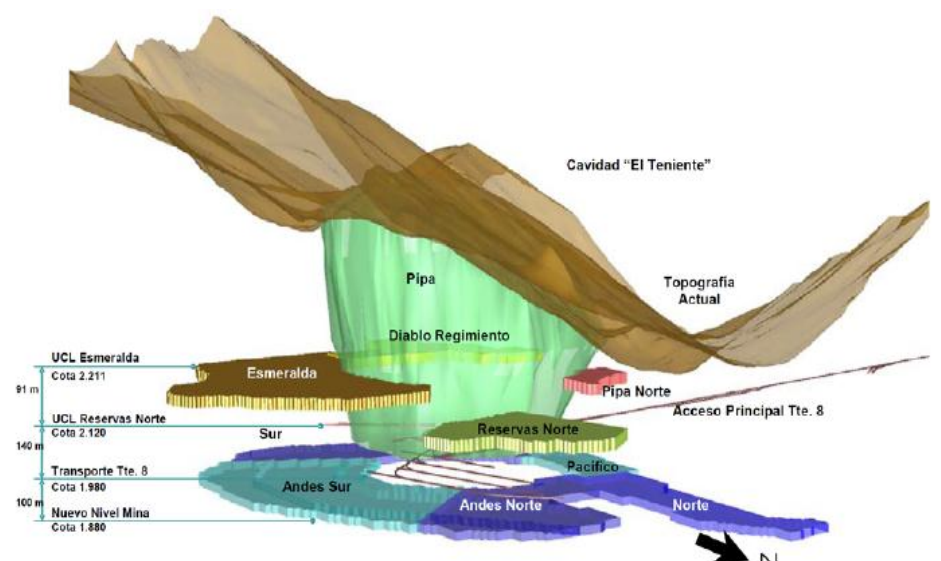
\includegraphics[width=400pt]{img/teniente.png}
    \caption{3D view of the different levels and mines in El Teniente Division \cite{baraona}}
    \label{fig:teniente}
\end{figure}


The exploitation occurs around this formation, where the mineralization gave place to 3 different zones:
\begin{enumerate}
    \item \emph{Sterile overload:} Located on the top of the deposit, it consists of different copper oxides, considered sterile since El Teniente only exploits sulphurs. 
    \item \emph{Secondary mineralization:} Located under the overload, it's a rich zone with a copper content of approximately $1.8\%$. This rock is easily fragmented, so the Block Caving method with manual extraction and gravitational transfer can be used.
    \item \emph{Primary mineralization:} Located under the secondary ore, it shows an important $50\%$ decrease in its copper content, and is defined as hard rock. This requires a mechanization of the extraction process, using Block Caving with LHDs (\emph{Load Haul Dump} machines) for extraction. Though this formation is more expensive to exploit, its big extension -running over 1000m below the lower level of El Teniente (Teniente 8)- makes it one of the biggest copper reserves in the world.
\end{enumerate}

The current extraction takes place in the primary mineralization, therefore LHDs are a necessity in the extracting area. To orchestrate the process, Block Caving and Panel Caving methods are used to 



\subsection{Scenario and mobility}

The scenario of an underground mine depends very much on the 

\subsection{Hypothesis and Generalizations}

\subsection{Extractive area model}





En este caso, consideraremos principalmente el nivel de extracción de una mina, donde se cuenta con vehículos que ingresan y salen del área cívica. Estos vehículos constan de acumulaciones de nodos, pero también son un nodo en sí mismos.

Luego de dejar a los otros nodos, los vehículos se van. Se tiene el centro cívico, que es el lugar donde los supervisores salen a dar rondas, y de donde todos los nodos, excepto los LHDs, van y vuelven.

La jornada de trabajo consiste en tener supervisores que dan rondas, y operarios que manejan las máquinas realizando circuitos entre el área de explotación y el área de chancado primario.

Consideraremos también grupos de mineros que van a puntos particulares del mapa, trabajan ahí en un rango pequeño, y luego vuelven al centro cívico.

Así podemos adaptar el escenario de desastre tal que tengamos las siguientes zonas:

Entrada al centro cívico
Interior centro cívico: 
Explotación: movimiento circular de las máquinas, rápidas (Nstat), movimiento aleatorio de nodos desde el centro cívico (.
Mantenimiento: La gente va, se queda ahí un rato, vuelve al centro cívico.

Para simular escenarios de minería, tomaremos como referencia el modelo de desastre 


\section*{Mining Scenario}

El siguiente escenario propone 

Zonas: OT, CC, OP, PR
Nodos: personas, vehiculos, LHDs
Tipo: transporte, estáticos




\bibliographystyle{plain}
\bibliography{comp.bib}

\end{document}